% !TeX encoding = UTF-8
% !TeX program = xelatex
% !TeX spellcheck = en_US

\documentclass[degree=bachelor]{thuthesis}
  % 学位 degree:
  %   doctor | master | bachelor | postdoc
  % 学位类型 degree-type:
  %   academic(默认)| professional
  % 语言 language
  %   chinese(默认)| english
  % 字体库 fontset
  %   windows | mac | fandol | ubuntu
  % 建议终版使用 Windows 平台的字体编译


% 论文基本配置,加载宏包等全局配置
% !TeX root = ./thuthesis-example.tex

% 论文基本信息配置

\thusetup{
  %******************************
  % 注意:
  %   1. 配置里面不要出现空行
  %   2. 不需要的配置信息可以删除
  %   3. 建议先阅读文档中所有关于选项的说明
  %******************************
  %
  % 输出格式
  %   选择打印版(print)或用于提交的电子版(electronic),前者会插入空白页以便直接双面打印
  %
  output = print,
  % 格式类型
  %   默认为论文(thesis),也可以设置为开题报告(proposal)
  % thesis-type = proposal,
  %
  % 标题
  %   可使用"\\"命令手动控制换行
  %
  title  = {清华大学学位论文 \LaTeX{} 模板\\使用示例文档 v\version},
  title* = {An Introduction to \LaTeX{} Thesis Template of Tsinghua
            University v\version},
  %
  % 学科门类
  %   1. 学术型
  %      - 中文
  %        需注明所属的学科门类,例如:
  %        哲学、经济学、法学、教育学、文学、历史学、理学、工学、农学、医学、
  %        军事学、管理学、艺术学
  %      - 英文
  %        博士:Doctor of Philosophy
  %        硕士:
  %          哲学、文学、历史学、法学、教育学、艺术学门类,公共管理学科
  %          填写"Master of Arts"",其它填写"Master of Science"
  %   2. 专业型
  %      直接填写专业学位的名称,例如:
  %      教育博士、工程硕士等
  %      Doctor of Education, Master of Engineering
  %   3. 本科生不需要填写
  %
  % degree-category  = {工学硕士},
  % degree-category* = {Master of Science},
  %
  % 培养单位
  %   填写所属院系的全名
  %
  department = {软件学院},
  %
  % 学科
  %   1. 研究生学术型学位,获得一级学科授权的学科填写一级学科名称,其他填写二级学科名称
  %   2. 本科生填写专业名称,第二学位论文需标注"(第二学位)"
  %
  discipline  = {软件工程},
  discipline* = {Software Engineering},
  %
  % 专业领域
  %   1. 设置专业领域的专业学位类别,填写相应专业领域名称
  %   2. 2019 级及之前工程硕士学位论文,在 `engineering-field` 填写相应工程领域名称
  %   3. 其他专业学位类别的学位论文无需此信息
  %
  % professional-field  = {计算机技术},
  % professional-field* = {Computer Technology},
  %
  % 姓名
  %
  author  = {陈敬文},
  author* = {Chen Ching-Wen},
  %
  % 学号
  % 仅当书写开题报告时需要(同时设置 `thesis-type = proposal')
  %
  % student-id = {2000310000},
  %
  % 指导教师
  %   中文姓名和职称之间以英文逗号","分开,下同
  %
  supervisor  = {刘璘, 研究员},
  supervisor* = {Researcher Liu Lin},
  %
  % 副指导教师
  %
  % associate-supervisor  = {陈文光, 教授},
  % associate-supervisor* = {Professor Chen Wenguang},
  %
  % 联合指导教师
  %
  % co-supervisor  = {某某某, 教授},
  % co-supervisor* = {Professor Mou Moumou},
  %
  % 日期
  %   使用 ISO 格式;默认为当前时间
  %
  % date = {2019-07-07},
  %
  % 是否在中文封面后的空白页生成书脊(默认 false)
  %
  include-spine = false,
  %
  % 密级和年限
  %   秘密, 机密, 绝密
  %
  % secret-level = {秘密},
  % secret-year  = {10},
  %
  % 博士后专有部分
  %
  % clc                = {分类号},
  % udc                = {UDC},
  % id                 = {编号},
  % discipline-level-1 = {计算机科学与技术},  % 流动站(一级学科)名称
  % discipline-level-2 = {系统结构},          % 专业(二级学科)名称
  % start-date         = {2011-07-01},        % 研究工作起始时间
}

% 载入所需的宏包

% 定理类环境宏包
\usepackage{amsthm}
% 也可以使用 ntheorem
% \usepackage[amsmath,thmmarks,hyperref]{ntheorem}

\thusetup{
  %
  % 数学字体
  % math-style = GB,  % GB | ISO | TeX
  math-font  = xits,  % stix | xits | libertinus
}

% 可以使用 nomencl 生成符号和缩略语说明
% \usepackage{nomencl}
% \makenomenclature

% 表格加脚注
\usepackage{threeparttable}

% 表格中支持跨行
\usepackage{multirow}

% 固定宽度的表格。
% \usepackage{tabularx}

% 跨页表格
\usepackage{longtable}

% 算法
\usepackage{algorithm}
\usepackage{algorithmic}

% 量和单位
\usepackage{siunitx}

% 参考文献使用 BibTeX + natbib 宏包
% 顺序编码制
% \usepackage[sort]{natbib}
% \bibliographystyle{thuthesis-numeric}

% 著者-出版年制
% \usepackage{natbib}
% \bibliographystyle{thuthesis-author-year}

% 生命科学学院要求使用 Cell 参考文献格式(2023 年以前使用 author-date 格式)
% \usepackage{natbib}
% \bibliographystyle{cell}

% 本科生参考文献的著录格式
\usepackage[sort]{natbib}
\bibliographystyle{thuthesis-bachelor}

% 参考文献使用 BibLaTeX 宏包
% \usepackage[style=thuthesis-numeric]{biblatex}
% \usepackage[style=thuthesis-author-year]{biblatex}
% \usepackage[style=gb7714-2015]{biblatex}
% \usepackage[style=apa]{biblatex}
% \usepackage[style=mla-new]{biblatex}
% 声明 BibLaTeX 的数据库
% \addbibresource{ref/refs.bib}

% 定义所有的图片文件在 figures 子目录下
\graphicspath{{figures/}}

% 数学命令
\makeatletter
\newcommand\dif{%  % 微分符号
  \mathop{}\!%
  \ifthu@math@style@TeX
    d%
  \else
    \mathrm{d}%
  \fi
}
\makeatother

% 代码列表
\usepackage{listings}

% hyperref 宏包在最后调用
\usepackage{hyperref}



\begin{document}

% 封面
\maketitle

% 学位论文指导小组、公开评阅人和答辩委员会名单
% 本科生不需要
% !TeX root = ../thuthesis-example.tex

\begin{committee}[name={学位论文指导小组、公开评阅人和答辩委员会名单}]

  \newcolumntype{C}[1]{@{}>{\centering\arraybackslash}p{#1}}

  \section*{指导小组名单}

  \begin{center}
    \begin{tabular}{C{3cm}C{3cm}C{9cm}@{}}
      李XX & 教授     & 清华大学 \\
      王XX & 副教授   & 清华大学 \\
      张XX & 助理教授 & 清华大学 \\
    \end{tabular}
  \end{center}


  \section*{公开评阅人名单}

  \begin{center}
    \begin{tabular}{C{3cm}C{3cm}C{9cm}@{}}
      刘XX & 教授   & 清华大学                    \\
      陈XX & 副教授 & XXXX大学                    \\
      杨XX & 研究员 & 中国XXXX科学院XXXXXXX研究所 \\
    \end{tabular}
  \end{center}


  \section*{答辩委员会名单}

  \begin{center}
    \begin{tabular}{C{2.75cm}C{2.98cm}C{4.63cm}C{4.63cm}@{}}
      主席 & 赵XX                  & 教授                    & 清华大学       \\
      委员 & 刘XX                  & 教授                    & 清华大学       \\
          & \multirow{2}{*}{杨XX} & \multirow{2}{*}{研究员} & 中国XXXX科学院 \\
          &                       &                         & XXXXXXX研究所  \\
          & 黄XX                  & 教授                    & XXXX大学       \\
          & 周XX                  & 副教授                  & XXXX大学       \\
      秘书 & 吴XX                  & 助理研究员              & 清华大学       \\
    \end{tabular}
  \end{center}

\end{committee}



% 也可以导入 Word 版转的 PDF 文件
% \begin{committee}[file=figures/committee.pdf]
% \end{committee}


% 使用授权的说明
% 本科生开题报告不需要
\copyrightpage
% 将签字扫描后授权文件 scan-copyright.pdf 替换原始页面
% \copyrightpage[file=scan-copyright.pdf]

\frontmatter
% !TeX root = ../thuthesis-example.tex

% 中英文摘要和关键字

\begin{abstract}
  TODO
  论文的摘要是对论文研究内容和成果的高度概括。
  摘要应对论文所研究的问题及其研究目的进行描述,对研究方法和过程进行简单介绍,对研究成果和所得结论进行概括。
  摘要应具有独立性和自明性,其内容应包含与论文全文同等量的主要信息。
  使读者即使不阅读全文,通过摘要就能了解论文的总体内容和主要成果。

  论文摘要的书写应力求精确、简明。
  切忌写成对论文书写内容进行提要的形式,尤其要避免“第 1 章……;第 2 章……;……”这种或类似的陈述方式。

  关键词是为了文献标引工作、用以表示全文主要内容信息的单词或术语。
  关键词不超过 5 个,每个关键词中间用分号分隔。

  % 关键词用“英文逗号”分隔,输出时会自动处理为正确的分隔符
  \thusetup{
    keywords = {关键词 1, 关键词 2, 关键词 3, 关键词 4, 关键词 5},
  }
\end{abstract}

\begin{abstract*}
  An abstract of a dissertation is a summary and extraction of research work and contributions.
  Included in an abstract should be description of research topic and research objective, brief introduction to methodology and research process, and summary of conclusion and contributions of the research.
  An abstract should be characterized by independence and clarity and carry identical information with the dissertation.
  It should be such that the general idea and major contributions of the dissertation are conveyed without reading the dissertation.

  An abstract should be concise and to the point.
  It is a misunderstanding to make an abstract an outline of the dissertation and words “the first chapter”, “the second chapter” and the like should be avoided in the abstract.

  Keywords are terms used in a dissertation for indexing, reflecting core information of the dissertation.
  An abstract may contain a maximum of 5 keywords, with semi-colons used in between to separate one another.

  % Use comma as separator when inputting
  \thusetup{
    keywords* = {keyword 1, keyword 2, keyword 3, keyword 4, keyword 5},
  }
\end{abstract*}


% 目录
\tableofcontents

% 插图和附表清单
% 本科生的插图索引和表格索引需要移至正文之后、参考文献前
% \listoffiguresandtables  % 插图和附表清单(仅限研究生)
\listoffigures           % 插图清单
\listoftables            % 附表清单

% 符号对照表
% !TeX root = ../thuthesis-example.tex

\begin{denotation}[3cm]
  \item[LLM] 大型语言模型(Large Language Model)
  \item[IDE] 集成开发环境(Integrated Development Environment)
  \item[CI/CD] 持续集成/持续部署(Continuous Integration/Continuous Deployment)
  \item[TDD] 测试驱动开发(Test-Driven Development)
  \item[API] 应用程序编程接口(Application Programming Interface)
  \item[API-first] API 优先开发(API-First Development)
  \item[MCP] 模型上下文协议(Model Context Protocol)
  \item[SSE] 服务器发送事件(Server-Sent Events)
\end{denotation}



% 也可以使用 nomencl 宏包,需要在导言区
% \usepackage{nomencl}
% \makenomenclature

% 在这里输出符号说明
% \printnomenclature[3cm]

% 在正文中的任意为都可以标题
% \nomenclature{PI}{聚酰亚胺}
% \nomenclature{MPI}{聚酰亚胺模型化合物,N-苯基邻苯酰亚胺}
% \nomenclature{PBI}{聚苯并咪唑}
% \nomenclature{MPBI}{聚苯并咪唑模型化合物,N-苯基苯并咪唑}
% \nomenclature{PY}{聚吡咙}
% \nomenclature{PMDA-BDA}{均苯四酸二酐与联苯四胺合成的聚吡咙薄膜}
% \nomenclature{MPY}{聚吡咙模型化合物}
% \nomenclature{As-PPT}{聚苯基不对称三嗪}
% \nomenclature{MAsPPT}{聚苯基不对称三嗪单模型化合物,3,5,6-三苯基-1,2,4-三嗪}
% \nomenclature{DMAsPPT}{聚苯基不对称三嗪双模型化合物(水解实验模型化合物)}
% \nomenclature{S-PPT}{聚苯基对称三嗪}
% \nomenclature{MSPPT}{聚苯基对称三嗪模型化合物,2,4,6-三苯基-1,3,5-三嗪}
% \nomenclature{PPQ}{聚苯基喹噁啉}
% \nomenclature{MPPQ}{聚苯基喹噁啉模型化合物,3,4-二苯基苯并二嗪}
% \nomenclature{HMPI}{聚酰亚胺模型化合物的质子化产物}
% \nomenclature{HMPY}{聚吡咙模型化合物的质子化产物}
% \nomenclature{HMPBI}{聚苯并咪唑模型化合物的质子化产物}
% \nomenclature{HMAsPPT}{聚苯基不对称三嗪模型化合物的质子化产物}
% \nomenclature{HMSPPT}{聚苯基对称三嗪模型化合物的质子化产物}
% \nomenclature{HMPPQ}{聚苯基喹噁啉模型化合物的质子化产物}
% \nomenclature{PDT}{热分解温度}
% \nomenclature{HPLC}{高效液相色谱(High Performance Liquid Chromatography)}
% \nomenclature{HPCE}{高效毛细管电泳色谱(High Performance Capillary lectrophoresis)}
% \nomenclature{LC-MS}{液相色谱-质谱联用(Liquid chromatography-Mass Spectrum)}
% \nomenclature{TIC}{总离子浓度(Total Ion Content)}
% \nomenclature{\textit{ab initio}}{基于第一原理的量子化学计算方法,常称从头算法}
% \nomenclature{DFT}{密度泛函理论(Density Functional Theory)}
% \nomenclature{$E_a$}{化学反应的活化能(Activation Energy)}
% \nomenclature{ZPE}{零点振动能(Zero Vibration Energy)}
% \nomenclature{PES}{势能面(Potential Energy Surface)}
% \nomenclature{TS}{过渡态(Transition State)}
% \nomenclature{TST}{过渡态理论(Transition State Theory)}
% \nomenclature{$\increment G^\neq$}{活化自由能(Activation Free Energy)}
% \nomenclature{$\kappa$}{传输系数(Transmission Coefficient)}
% \nomenclature{IRC}{内禀反应坐标(Intrinsic Reaction Coordinates)}
% \nomenclature{$\nu_i$}{虚频(Imaginary Frequency)}
% \nomenclature{ONIOM}{分层算法(Our own N-layered Integrated molecular Orbital and molecular Mechanics)}
% \nomenclature{SCF}{自洽场(Self-Consistent Field)}
% \nomenclature{SCRF}{自洽反应场(Self-Consistent Reaction Field)}



% 正文部分
\mainmatter
% !TeX root = ../thuthesis-example.tex

\chapter{引言与研究背景}

\section{研究背景与意义}
近年来,大语言模型(Large Language Models, LLMs)在代码生成领域展现出显著进步,成为自然语言与可执行代码之间桥梁能力提升的重要驱动力。相关系统性综述表明,LLM 在 HumanEval、MBPP 等主流基准任务中的表现持续提升,反映出模型在理解与生成能力上的重大突破\cite{jiang2024survey}。同时,学界也在不断完善对代码生成准确性、效率及可读性的评测方法,推动评测体系向更高标准发展\cite{chen2024eval}。在工业界,AI 编程辅助工具的应用快速普及。GitHub 的调研数据显示,92\% 的美国开发者已在实际开发中采用此类工具\cite{githubblog2023};SWE-bench 评测中 LLM 的问题解决率已从 2023 年的 4.4\% 显著提升至 69.1\%,进一步印证了 AI 驱动开发效率的提升\cite{ft2025ai}。

尽管 LLM 相关研究和应用持续取得突破,如何将其能力真正融入大型软件工程实践,仍面临诸多挑战,包括上下文理解受限、反馈机制不完善以及工程化流程缺失等。因此,将 LLM 的生成能力与软件工程最佳实践紧密结合,如测试驱动开发(Test-Driven Development, TDD)、API 优先(API-First)开发和持续集成/持续部署(Continuous Integration/Continuous Deployment, CI/CD),已成为当前亟待解决的重要课题。

\section{当前 LLM 辅助开发工具发展与挑战}

为系统梳理主流 LLM 编程工具在实际开发环境中的差异,表~\ref{tab:llm-tools-updated} 汇总了几款代表性产品在集成平台、主要功能及反馈机制方面的对比。当前具有影响力的典型工具包括 GitHub Copilot X、Cursor、v0.dev、Replit、Lovable、Windsurf 和 bolt.new 等。


\begin{table}[H]
  \centering
  \footnotesize
  \caption{典型 LLM 辅助开发工具功能对比}
  \label{tab:llm-tools-updated}
  \setlength{\tabcolsep}{3pt}
  \begin{tabular}{
    >{\raggedright\arraybackslash}p{2.4cm}
    >{\raggedright\arraybackslash}p{2.6cm}
    >{\raggedright\arraybackslash}p{3.6cm}
    >{\raggedright\arraybackslash}p{4.6cm}
  }
    \toprule
    \textbf{工具名称} & \textbf{集成平台} & \textbf{主要功能} & \textbf{反馈机制} \\
    \midrule
    GitHub Copilot\cite{copilotx2023}      & VS Code/JetBrains 扩展        & 多模型(GPT-4o、Claude 3.5、Gemini 1.5 Pro)行内补全、代码审查支持      & 无内置 CI 流水线反馈                                \\
    \addlinespace
    Cursor\cite{cursor2025wiki}            & 独立 AI IDE(VS Code 分支)    & 对话式多文件生成、跨文件重构、Diff 视图              & 实时代码差异预览;无原生 TDD/CI/CD 集成            \\
    \addlinespace
    v0.dev\cite{v0dev2024}                 & 浏览器内 Chat UI               & 基于 React/Tailwind 的 UI 自动生成                  & 页面预览与即时部署;缺少测试与流水线支持            \\
    \addlinespace
    Replit\cite{replit2025wiki}            & 云端 IDE                       & Ghostwriter AI、Agent V2 对话式生成、协同编辑       & 实时代码运行、部署管道;无结构化测试反馈            \\
    \addlinespace
    Lovable\cite{lovable2025times}         & Web App Builder                & 对话式前后端+数据库一体化生成                      & 即时预览与调试;无原生 CI/CD 流水线                \\
    \addlinespace
    Windsurf\cite{windsurf2024}            & AI 增强 IDE                    & 行内补全、多文件编辑、聊天问答                      & 变更高亮与上下文聊天;尚无 TDD/CI 插件            \\
    \addlinespace
    bolt.new\cite{arunachalam2024boltnew,boltnewgithub2024} & 浏览器 IDE(StackBlitz WebContainers) & 从提示到部署:项目依赖管理、Node.js 运行、前后端一体化生成 & 终端输出、即时预览与部署状态反馈;支持文件系统与第三方 API 调用 \\
    \bottomrule
  \end{tabular}
\end{table}

GitHub Copilot X 自 2023 年起,在多模型切换和多文件补全方面取得了显著进展,集成了 GPT-4o、Claude 3.5 和 Gemini 1.5 Pro,支持基于项目全局上下文的代码建议生成,并新增了代码审查和安全提示等能力,但与 CI/CD 或 TDD 流程的深度集成仍有待加强\cite{copilotx2023}。Cursor 通过"vibe coding"工作流,将对话式多文件生成与实时 Diff 视图结合,提升了多文件协同开发效率。然而,其自动化测试和持续交付方案尚不完整,部分流程仍需借助外部工具补充\cite{cursor2025wiki}。v0.dev 主打对话生成 React/Tailwind 前端代码和一键部署,适合原型设计及 UI 快速验证,但缺乏对测试的原生支持\cite{v0dev2024}。Replit 借助 Ghostwriter AI 和 Agent V2,实现了云端协作开发与即时运行体验,但结构化测试和 CI/CD 功能仍主要依赖外部插件\cite{replit2025wiki}。Lovable 能在单轮对话中生成全栈前后端与数据库代码,支持即时预览,但缺乏完善的版本控制与自动化流水线,难以满足团队长期协作需求\cite{lovable2025times}。Windsurf 将行内补全与上下文对话结合,提升代码建议的语义丰富性,但暂未实现与 TDD 或 CI/CD 的深度耦合\cite{windsurf2024}。bolt.new 依托 StackBlitz WebContainers,提供浏览器内完整的依赖安装、Node.js 服务与代码生成能力,终端输出和部署状态反馈为快速验证提供便利,但在测试驱动和持续交付方面仍有扩展空间\cite{arunachalam2024boltnew,boltnewgithub2024}。

可以看到,尽管上述工具在各自领域取得了一定进展,但在应用于实际软件工程实践中仍存在几项关键挑战:

\subsection{上下文理解局限}

在处理大型与复杂软件代码库时,当前工具面临对代码上下文理解不足的问题。GitHub Copilot 等早期工具主要基于当前打开的文件内容进行补全,对项目全局信息缺乏深入理解。即使是 Cursor 和 Windsurf 等支持多文件编辑的工具,在理解代码模块间接口关系、命名规范以及整体架构设计约定等方面仍有不足,导致生成的代码难以与既有环境高效融合。

\subsection{交互反馈与即时验证不足}

现有工具普遍缺乏完整、成熟的网页端实时代码运行及预览能力,使开发人员难以即时观察和验证生成代码的实际表现。虽然 bolt.new 通过 WebContainers 提供了浏览器内运行环境,v0.dev 和 Lovable 支持 UI 代码即时预览,但它们在复杂项目的测试验证方面仍不完善。多数平台尚未实现生成代码的即时测试反馈,依赖与配置问题难以及时被发现和解决,开发流程中从代码生成到测试验证的环节也未能做到无缝衔接,用户体验仍然割裂。

\subsection{软件工程实践融合不足}

当前 LLM 辅助工具尚未有效整合现代软件工程的最佳实践。尽管 Replit 提供了部分部署管道,但对于测试驱动开发、API 优先设计以及持续集成与部署等核心流程的支持仍显不足。这种融合上的欠缺,导致工具在多个方面存在局限。首先,缺乏基于测试定义指导代码生成的系统化方法,使开发过程难以保证质量可控。其次,API 开发过程中规范定义与实现往往相互割裂,难以确保一致性和可维护性。最后,从代码生成到部署的全链路自动化程度较低,仍需开发者投入大量人工操作,难以实现高效闭环。这些问题共同凸显了一个系统化软件工程环境的必要性,即不仅要充分发挥 LLM 在代码生成方面的能力,还应将其与软件工程最佳实践紧密结合,形成覆盖需求定义、代码验证到系统部署的完整开发流程。

\section{bolt.SE的目标}

基于以上分析,本研究提出了面向无代码基础用户与编程初学者的交互式软件开发环境——bolt.SE。其中,"bolt"来源于开源项目bolt.diy,体现该平台的技术基础;"SE"则表示软件工程(Software Engineering),突出该环境对软件工程方法论的深度融合与系统化支持。

bolt.SE旨在将大语言模型的自然语言处理与代码生成优势,与现代软件工程领域公认的最佳实践深度融合,实现更加高效且易用的LLM驱动软件原型开发工具。具体目标包括:

\begin{itemize}
    \item 系统引入API优先开发模块,增强LLM与外部服务的交互能力。通过基于OpenAPI规范的API定义与管理,让LLM理解并生成符合API规范的代码,实现外部服务与LLM的无缝对接,有效扩展模型功能边界。
    \item 通过结构化的测试驱动开发模块,改善代码生成质量与可靠性。该模块让用户能够在生成代码前先定义期望行为,将测试约束转化为LLM可理解的指导信息,建立基于"红-绿-重构"循环的验证机制,确保生成代码符合预定义行为。
    \item 通过模型上下文协议(MCP)模块,突破LLM知识与功能边界。此模块提供标准化接口,支持LLM安全调用外部工具和数据源,实现访问远程服务调用的多场景支持。
    \item 通过MCP与TDD协同实现CI/CD自动化流程,完成从测试定义到部署的全链路自动化。系统利用标准化工具接口自动完成仓库创建、配置生成、代码推送与流水线触发等操作,形成完整开发闭环,简化传统手动操作环节。
\end{itemize}

这些目标共同构成一个端到端软件开发环境,使开发者能够专注于创意表达与业务逻辑,而非繁琐的编程细节,提高软件原型设计与开发的可达性与效率。

本研究将基于bolt.diy开源框架构建bolt.SE平台,实现对API优先开发、测试驱动开发与模型上下文协议等核心技术模块的集成,以达到前述目标。

\section{论文结构}
论文结构安排如下:

第1章(本章)介绍研究背景、问题提出与目标,分析当前LLM辅助开发工具的发展与挑战,概述bolt.SE的核心设计。

第\ref{chap:code-generation}章详细介绍bolt.SE系统的整体架构、核心技术及创新点。该章首先介绍bolt.diy的基础架构与技术特点,包括开源与扩展性、多种大语言模型支持、代码生成能力以及WebContainer技术等方面。随后重点阐述bolt.SE的创新模块及其在软件工程流程中的应用价值,包括API优先开发模块、测试驱动开发模块和模型上下文协议模块。

第\ref{chap:api-first}章聚焦API优先开发模块,介绍OpenAPI规范在bolt.SE中的应用,API定义与管理机制,以及LLM如何理解并调用API实现功能扩展。该章将分析bolt.SE中APIActions的实现方案,展示结构化API定义如何帮助LLM突破知识局限,通过与外部服务交互扩展其能力边界。

第\ref{chap:tdd}章详细阐述测试驱动开发模块的概念与技术实现,分析TDD在LLM驱动开发中的价值,并通过具体案例展示测试定义如何引导LLM生成高质量代码。该章将介绍bolt.SE测试功能的技术实现,并通过JavaScript计算器的开发流程,展示基于"红–绿–重构"循环的测试驱动开发过程。

第\ref{chap:mcp}章深入剖析模型上下文协在bolt.SE中的原理与实现,分析MCP如何通过标准化工具接口使LLM能够安全地访问外部资源,突破知识截止限制,降低输出幻觉风险,并支持实时数据获取与专业工具调用。通过IoTDB数据库集成案例,展示MCP在统一自然语言交互中同时发现并调用多类工具的强大能力。

第\ref{chap:mcp-tdd-cicd}章综合前述核心技术,展示MCP与TDD协同驱动的GitLab CI/CD自动化流程,体现bolt.SE在全链路软件工程实践中的系统集成能力。该章通过应用实例,详述从Jest测试定义到GitLab仓库创建、CI配置自动生成及部署的完整开发闭环,实现从测试、代码、仓库、流水线到部署的全链路自动化。

第\ref{chap:conclusion}章总结全文研究成果,阐述bolt.SE与bolt.diy开源项目的紧密联系和相互促进的创新循环,以及对社区的贡献。同时展望bolt.SE的应用潜力与未来计划。
% !TeX root = ../thuthesis-example.tex

% TODO: papers
% https://github.com/FudanSELab/Agent4SE-Paper-List
% Multi-Programming Language Sandbox for LLMs https://arxiv.org/pdf/22410.23074
% Planning-Driven Programming https://arxiv.org/pdf/2411.14503
% AutoDev https://arxiv.org/pdf/2403.08299


\chapter{文献综述}

\section{}


% !TeX root = ../thuthesis-example.tex
\chapter{bolt.SE 介绍}

本项目基于开源项目bolt.diy(以下简称bolt),在此基础上进行了多方面的优化和扩展。选择bolt作为基础平台的原因主要体现在以下几个方面:

\section{选择bolt的原因}

\begin{itemize}
    \item \textbf{开源与扩展性}: bolt作为一个开源平台,具备高度的扩展性和灵活性,便于根据项目的需求进行定制化开发,适应各种软件工程实践的要求。
    \item \textbf{多种大语言模型支持}: bolt支持多种大语言模型(LLM),如GPT-o3-mini、Claude 3.7 Sonnet等,且持续扩展对新模型的支持,这为代码生成提供了更多选择,极大地增强了系统的灵活性。
    \item \textbf{代码生成能力}: bolt具备出色的代码生成能力,尤其擅长理解和感知大规模复杂软件项目的上下文信息,在解析代码库和管理项目结构方面表现卓越。
    \item \textbf{WebContainer技术}: bolt使用WebContainer技术,使得代码能在浏览器中实时执行并预览,极大提升了开发的交互性和实时响应能力,便于开发者快速验证代码效果。
\end{itemize}

\section{系统整体流程}

bolt系统的流程图如图~\ref{fig:general_chat_sequence}所示。该图展示了从用户提交需求到最终生成并执行代码的完整流程。

\begin{figure}[ht]
  \centering
  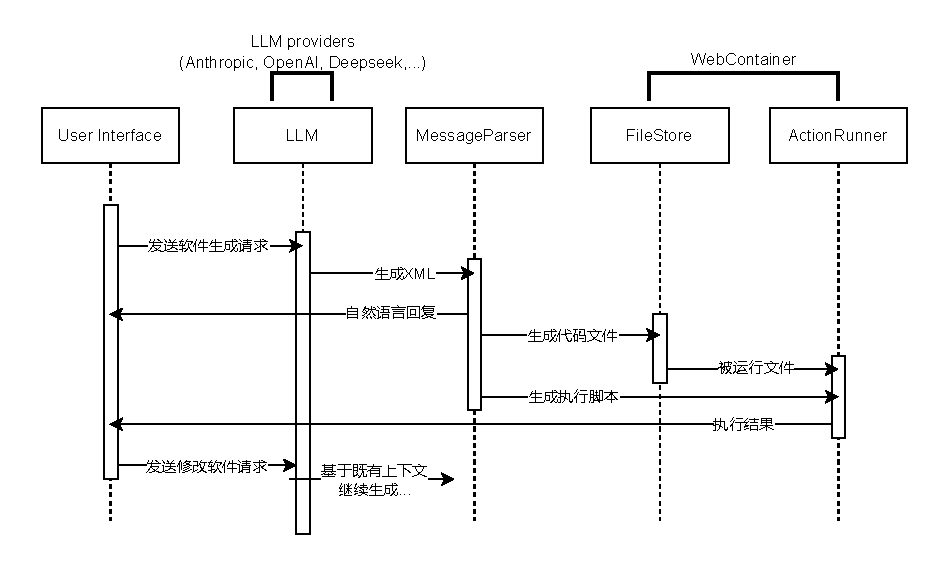
\includegraphics[width=1.0\linewidth]{general_chat_sequence.drawio.pdf}
  \caption{bolt.SE 代码生成时序图}
  \label{fig:general_chat_sequence}
\end{figure}

系统的整体流程包括以下几个关键步骤:
\begin{itemize}
    \item 用户通过UI界面输入需求,选择适当的大语言模型(LLM)。
    \item LLM生成自然语言响应,经过MessageParser模块解析为结构化XML格式。
    \item 生成的代码通过FileStore存储,并通过ActionRunner在WebContainer环境中执行。
    \item 执行结果通过ActionRunner反馈给用户,完成代码生成和执行过程。
\end{itemize}

其中,ActionRunner、FileStore 和 WebContainer 进行交互,WebContainer 提供了一个隔离、安全的运行环境,允许代码在浏览器中直接执行。WebContainer 的具体实现原理将在后续章节中详细介绍。

\section{UI与操作流程介绍}

bolt提供了一个直观易用的用户界面(UI),用户可以通过该界面方便地输入需求、选择模型、查看代码生成结果并进行进一步编辑。

\subsection{用户需求输入与模型选择}

用户在UI的左侧输入自然语言描述软件功能需求。bolt平台支持多种大语言模型(如OpenAI、Anthropic、DeepSeek等),用户可以根据需求选择适合的模型,以优化代码生成效果。

\subsection{代码生成与编辑}

根据用户输入的需求,bolt会自动调用选定的LLM生成代码,生成的代码会在在线IDE中展示。用户可以在IDE中进一步编辑、修改代码,并通过实时语法检查和错误提示功能及时发现问题。

\subsection{实时预览与调试}

bolt的WebContainer技术允许用户在浏览器中实时运行和预览生成的代码,开发者无需离开开发环境,即可直接验证代码的功能和效果。

\section{LLM介绍}

大语言模型(LLM)在本项目中的核心作用是生成代码并持续记忆上下文信息。以下分别介绍LLM在本项目中的应用及其优势。

\subsection{多LLM支持及其好处}

bolt支持多种LLM的接入,包括GPT-o3-mini、Claude 3.7 Sonnet等,未来还将进一步扩展对新模型的支持。具体而言,bolt内部已对多种LLM提供商的API进行了封装,用户只需向各平台申请API Key,并配置在系统中,即可使用对应的模型。
这一多模型支持的优势在于:
\begin{itemize}
    \item 用户可以根据具体的项目需求,选择最适合的模型,优化代码生成效果。
    \item 通过灵活切换模型,能够适应不同的代码生成任务,如前端开发、后端开发等,提供更好的定制化能力。
    \item 多模型支持减少对单一模型的依赖,避免出现由于某个模型的缺陷或更新导致的不可用情况。
\end{itemize}

\subsection{大语言模型的超长文本处理能力}

传统的代码生成工具,如GitHub Copilot、Cursor和DeepSeek等,通常在生成代码时只关注当前输入的单一上下文片段或局限于当前编辑区域附近的上下文。这导致当代码库规模增大时,生成的代码可能缺乏一致性,或忽略已有代码库的风格和约定。

而在bolt平台中,由于所有的代码生成过程本质上都表现为用户与大语言模型之间一来一往的交互对话,因此,整个项目的代码库实际上就是一系列高度结构化的“对话记录”。利用LLM的超长文本处理能力,bolt能够将这些累积的对话历史完整地纳入模型的记忆上下文。这种独特的设计使LLM不仅能基于当前用户输入生成代码,还能够回顾并记忆历史生成的代码片段、开发者的设计决策以及代码库整体的架构约定。

\section{MessageParser}

MessageParser是系统中的一个关键模块,负责将大语言模型(LLM)生成的自然语言响应解析为结构化的数据格式,通常是XML格式。该XML格式不仅包含生成的代码,还包括后续的操作步骤、文件路径等信息,能够高效地支持后续的代码生成和执行等任务。下面以一个创建JavaScript函数的例子来详细说明XML结构的组成及其各标签的功能。

\subsection{Prompt定义的XML结构}

为了便于MessageParser解析和处理LLM的输出,我们设计了一个特定的XML结构。该结构能够清晰地表达每一步生成的代码和执行的操作。以下是一个例子,展示了如何通过XML结构描述一个创建JavaScript函数的过程:

\begin{lstlisting}[breaklines=true,basicstyle=\ttfamily\small]
<example>
  <user_query>Can you help me create a JavaScript function to calculate the factorial of a number?</user_query>
  <assistant_response>
    Certainly, I can help you create a JavaScript function to calculate the factorial of a number.

    <boltArtifact id="factorial-function" title="JavaScript Factorial Function">
      <boltAction type="file" filePath="index.js">
        function factorial(n) {
          return n <= 1 ? 1 : n * factorial(n - 1);
        }
      </boltAction>

      <boltAction type="shell">node index.js</boltAction>
    </boltArtifact>
  </assistant_response>
</example>
\end{lstlisting}

\subsubsection{XML标签说明}

这个XML结构中,主要涉及以下几个标签和子标签:

\begin{itemize}
    \item \textbf{\textless user\_query\textgreater}: 该标签包含用户输入的自然语言查询。在本例中,用户请求创建一个计算阶乘的JavaScript函数。
    
    \item \textbf{\textless assistant\_response\textgreater}: 该标签包含LLM的自然语言响应。它不仅包括对用户查询的文本回复,还包括后续的操作步骤,通常是通过`boltArtifact`和`boltAction`来描述代码生成和执行的过程。
    
    \item \textbf{\textless boltArtifact\textgreater}: 这是一个容器标签,用于表示一个生成的代码单元或"工件"。在本例中,`boltArtifact`表示生成的JavaScript阶乘函数。它具有两个重要的属性:
    \begin{itemize}
        \item \textbf{id}: 唯一标识符,用于引用和管理生成的代码单元。
        \item \textbf{title}: 标题或描述,帮助用户理解该工件的内容。在此例中,标题是"JavaScript Factorial Function"。
    \end{itemize}
    
    \item \textbf{\textless boltAction\textgreater}: 这是描述具体操作的标签,它包含了代码生成、文件操作和执行指令等步骤。每个`boltAction`代表一个单独的操作,可以是文件生成、命令执行等。在本例中,`boltAction`有两种类型:
    \begin{itemize}
        \item \textbf{type="file"}: 表示这是一个文件操作,文件内容就是生成的JavaScript函数。`filePath`属性指定了文件的路径,这里是`index.js`,它是包含阶乘函数的文件。
        \item \textbf{type="shell"}: 表示这是一个命令行操作,`boltAction`标签中的内容是一个shell命令。在本例中,命令是`node index.js`,表示在命令行中运行生成的JavaScript文件。
    \end{itemize}
\end{itemize}

\subsubsection{如何处理XML结构}

在实际应用中,MessageParser会根据LLM的输出将自然语言响应转换为这种XML结构。每个操作步骤都会被封装成`boltAction`,而所有的操作步骤将组成一个`boltArtifact`,最终这些`boltArtifact`构成了完整的代码生成流程。

1. 用户的查询会被传递给LLM,LLM解析查询并生成自然语言响应(如上例中的JavaScript代码)。
2. MessageParser接收LLM的响应,并将其转换为结构化的XML数据,其中包含了生成的代码(如`factorial`函数)及相关操作(如创建文件和执行代码)。
3. 系统根据这些`boltArtifact`和`boltAction`执行相应的操作,如创建文件、执行命令等。

\subsection{结构化数据的优势}

通过将LLM生成的自然语言响应转化为结构化的XML格式,MessageParser能够高效地将生成的代码和操作步骤传递给后续模块,如FileStore和ActionRunner。这种结构化方式使得系统能够:
\begin{itemize}
    \item 高效地管理和执行多个代码生成和执行任务。
    \item 便于扩展和定制化,可以根据具体需求调整`boltAction`的类型和操作。
    \item 提供清晰的反馈和调试信息,帮助开发者快速定位问题。
\end{itemize}

总之,XML格式不仅是LLM与系统之间的桥梁,还能够促进后续操作的自动化和可管理性,从而提升整个系统的效率和可扩展性。

\section{WebContainer简介}

WebContainer 是由 StackBlitz 开发的基于 WebAssembly 的微型操作系统,旨在在浏览器中原生运行 Node.js 环境。它通过将 Node.js 编译为 WebAssembly(WASM),使开发者能够在浏览器中直接执行服务器端代码,如运行 Node.js 服务器、安装 npm 包等。 

\subsection{实现原理}

WebContainer 的核心在于利用 WebAssembly 技术,将 Node.js 及相关工具链编译为可在浏览器中运行的格式。具体而言,它在浏览器中模拟了一个完整的操作系统环境,包括文件系统和进程管理等功能。这使得开发者可以在浏览器中执行诸如 \texttt{npm install}、\texttt{node index.js} 等命令,实现完整的开发工作流程。 

\subsection{在 bolt 系统中的应用}

在 bolt 系统中,WebContainer 被用于提供一个安全、隔离的运行环境,以支持代码的生成和执行:

\begin{enumerate}

    \item 代码存储:生成的代码通过 FileStore 模块存储在 WebContainer 的虚拟文件系统中,确保代码资产的安全管理和版本控制。

    \item 代码执行:ActionRunner 模块从 FileStore 获取代码,并在 WebContainer 环境中执行。由于 WebContainer 提供了完整的 Node.js 运行时,代码可以在其中被直接运行。

    \item 结果反馈:执行结果通过 ActionRunner 返回给用户,并进行渲染。
\end{enumerate}

通过上述流程,bolt 系统利用 WebContainer 的能力,实现了在浏览器中直接进行代码的生成、存储、执行和反馈,使使用者能够实时看到代码的执行结果,极大地提升了开发效率和用户体验。 

TODO: 截图演示原始bolt.diy

\section{改进}

本项目在bolt的基础上,进行了以下改进:
TODO


% examples
% !TeX root = ../thuthesis-example.tex

\chapter{论文主要部分的写法}

研究生学位论文撰写,除表达形式上需要符合一定的格式要求外,内容方面上也要遵循一些共性原则。

通常研究生学位论文只能有一个主题(不能是几块工作拼凑在一起),该主题应针对某学科领域中的一个具体问题展开深入、系统的研究,并得出有价值的研究结论。
学位论文的研究主题切忌过大,例如,“中国国有企业改制问题研究”这样的研究主题过大,因为“国企改制”涉及的问题范围太广,很难在一本研究生学位论文中完全研究透彻。



\section{论文的语言及表述}

除国际研究生外,学位论文一律须用汉语书写。
学位论文应当用规范汉字进行撰写,除古汉语研究中涉及的古文字和参考文献中引用的外文文献之外,均采用简体汉字撰写。

国际研究生一般应以中文或英文书写学位论文,格式要求同上。
论文须用中文封面。

研究生学位论文是学术作品,因此其表述要严谨简明,重点突出,专业常识应简写或不写,做到立论正确、数据可靠、说明透彻、推理严谨、文字凝练、层次分明,避免使用文学性质的或带感情色彩的非学术性语言。

论文中如出现一个非通用性的新名词、新术语或新概念,需随即解释清楚。



\section{论文题目的写法}

论文题目应简明扼要地反映论文工作的主要内容,力求精炼、准确,切忌笼统。
论文题目是对研究对象的准确、具体描述,一般要在一定程度上体现研究结论,因此,论文题目不仅应告诉读者这本论文研究了什么问题,更要告诉读者这个研究得出的结论。
例如:“在事实与虚构之间:梅乐、卡彭特、沃尔夫的新闻观”就比“三个美国作家的新闻观研究”更专业、更准确。



\section{摘要的写法}

论文摘要是对论文研究内容的高度概括,应具有独立性和自含性,即应是 一篇简短但意义完整的文章。
通过阅读论文摘要,读者应该能够对论文的研究 方法及结论有一个整体性的了解,因此摘要的写法应力求精确简明。
论文摘要 应包括对问题及研究目的的描述、对使用的方法和研究过程进行的简要介绍、 对研究结论的高度凝练等,重点是结果和结论。

论文摘要切忌写成全文的提纲,尤其要避免“第 1 章……;第 2 章……;……”这样的陈述方式。



\section{引言的写法}

一篇学位论文的引言大致包含如下几个部分:
1、问题的提出;
2、选题背 景及意义;
3、文献综述;
4、研究方法;
5、论文结构安排。
\begin{itemize}
  \item 问题的提出:要清晰地阐述所要研究的问题“是什么”。
    \footnote{选题时切记要有“问题意识”,不要选不是问题的问题来研究。}
  \item 选题背景及意义:论述清楚为什么选择这个题目来研究,即阐述该研究对学科发展的贡献、对国计民生的理论与现实意义等。
  \item 文献综述:对本研究主题范围内的文献进行详尽的综合述评,“述”的同时一定要有“评”,指出现有研究状态,仍存在哪些尚待解决的问题,讲出自己的研究有哪些探索性内容。
  \item 研究方法:讲清论文所使用的学术研究方法。
  \item 论文结构安排:介绍本论文的写作结构安排。
\end{itemize}



\section{正文的写法}

本部分是论文作者的研究内容,不能将他人研究成果不加区分地掺和进来。
已经在引言的文献综述部分讲过的内容,这里不需要再重复。
各章之间要存在有机联系,符合逻辑顺序。



\section{结论的写法}

结论是对论文主要研究结果、论点的提炼与概括,应精炼、准确、完整,使读者看后能全面了解论文的意义、目的和工作内容。
结论是最终的、总体的结论,不是正文各章小结的简单重复。
结论应包括论文的核心观点,主要阐述作者的创造性工作及所取得的研究成果在本领域中的地位、作用和意义,交代研究工作的局限,提出未来工作的意见或建议。
同时,要严格区分自己取得的成果与指导教师及他人的学术成果。

在评价自己的研究工作成果时,要实事求是,除非有足够的证据表明自己的研究是“首次”、“领先”、“填补空白”的,否则应避免使用这些或类似词语。

% !TeX root = ../thuthesis-example.tex

\chapter{图表示例}

\section{插图}

图片通常在 \env{figure} 环境中使用 \cs{includegraphics} 插入,如图~\ref{fig:example} 的源代码。
建议矢量图片使用 PDF 格式,比如数据可视化的绘图;
照片应使用 JPG 格式;
其他的栅格图应使用无损的 PNG 格式。
注意,LaTeX 不支持 TIFF 格式;EPS 格式已经过时。

\begin{figure}
  \centering
  
\includegraphics[width=0.5\linewidth]{example-image-a.pdf}
  \caption*{国外的期刊习惯将图表的标题和说明文字写成一段,需要改写为标题只含图表的名称,其他说明文字以注释方式写在图表下方,或者写在正文中。}
  \caption{示例图片标题}
  \label{fig:example}
\end{figure}

若图或表中有附注,采用英文小写字母顺序编号,附注写在图或表的下方。
国外的期刊习惯将图表的标题和说明文字写成一段,需要改写为标题只含图表的名称,其他说明文字以注释方式写在图表下方,或者写在正文中。

如果一个图由两个或两个以上分图组成时,各分图分别以 (a)、(b)、(c)...... 作为图序,并须有分图题。
推荐使用 \pkg{subcaption} 宏包来处理, 比如图~\ref{fig:subfig-a} 和图~\ref{fig:subfig-b}。

\begin{figure}
  \centering
  \subcaptionbox{分图 A\label{fig:subfig-a}}
    {
\includegraphics[width=0.35\linewidth]{example-image-a.pdf}}
  \subcaptionbox{分图 B\label{fig:subfig-b}}
    {
\includegraphics[width=0.35\linewidth]{example-image-b.pdf}}
  \caption{多个分图的示例}
  \label{fig:multi-image}
\end{figure}



\section{表格}

表应具有自明性。为使表格简洁易读,尽可能采用三线表,如表~\ref{tab:three-line}。
三条线可以使用 \pkg{booktabs} 宏包提供的命令生成。

\begin{table}
  \centering
  \caption{三线表示例}
  \begin{tabular}{ll}
    \toprule
    文件名          & 描述                         \\
    \midrule
    thuthesis.dtx   & 模板的源文件,包括文档和注释 \\
    thuthesis.cls   & 模板文件                     \\
    thuthesis-*.bst & BibTeX 参考文献表样式文件    \\
    \bottomrule
  \end{tabular}
  \label{tab:three-line}
\end{table}

表格如果有附注,尤其是需要在表格中进行标注时,可以使用 \pkg{threeparttable} 宏包。
研究生要求使用英文小写字母 a、b、c……顺序编号,本科生使用圈码 ①、②、③……编号。

\begin{table}
  \centering
  \begin{threeparttable}[c]
    \caption{带附注的表格示例}
    \label{tab:three-part-table}
    \begin{tabular}{ll}
      \toprule
      文件名                 & 描述                         \\
      \midrule
      thuthesis.dtx\tnote{a} & 模板的源文件,包括文档和注释 \\
      thuthesis.cls\tnote{b} & 模板文件                     \\
      thuthesis-*.bst        & BibTeX 参考文献表样式文件    \\
      \bottomrule
    \end{tabular}
    \begin{tablenotes}
      \item [a] 可以通过 xelatex 编译生成模板的使用说明文档;
        使用 xetex 编译 \file{thuthesis.ins} 时则会从 \file{.dtx} 中去除掉文档和注释,得到精简的 \file{.cls} 文件。
      \item [b] 更新模板时,一定要记得编译生成 \file{.cls} 文件,否则编译论文时载入的依然是旧版的模板。
    \end{tablenotes}
  \end{threeparttable}
\end{table}

如某个表需要转页接排,可以使用 \pkg{longtable} 宏包,需要在随后的各页上重复表的编号。
编号后跟表题(可省略)和“(续)”,置于表上方。续表均应重复表头。

\begin{longtable}{cccc}
    \caption{跨页长表格的表题}
    \label{tab:longtable} \\
    \toprule
    表头 1 & 表头 2 & 表头 3 & 表头 4 \\
    \midrule
  \endfirsthead
    \caption*{续表~\thetable\quad 跨页长表格的表题} \\
    \toprule
    表头 1 & 表头 2 & 表头 3 & 表头 4 \\
    \midrule
  \endhead
    \bottomrule
  \endfoot
  Row 1  & & & \\
  Row 2  & & & \\
  Row 3  & & & \\
  Row 4  & & & \\
  Row 5  & & & \\
  Row 6  & & & \\
  Row 7  & & & \\
  Row 8  & & & \\
  Row 9  & & & \\
  Row 10 & & & \\
\end{longtable}



\section{算法}

算法环境可以使用 \pkg{algorithms} 或者 \pkg{algorithm2e} 宏包。

\renewcommand{\algorithmicrequire}{\textbf{输入:}\unskip}
\renewcommand{\algorithmicensure}{\textbf{输出:}\unskip}

\begin{algorithm}
  \caption{Calculate $y = x^n$}
  \label{alg1}
  \small
  \begin{algorithmic}
    \REQUIRE $n \geq 0$
    \ENSURE $y = x^n$

    \STATE $y \leftarrow 1$
    \STATE $X \leftarrow x$
    \STATE $N \leftarrow n$

    \WHILE{$N \neq 0$}
      \IF{$N$ is even}
        \STATE $X \leftarrow X \times X$
        \STATE $N \leftarrow N / 2$
      \ELSE[$N$ is odd]
        \STATE $y \leftarrow y \times X$
        \STATE $N \leftarrow N - 1$
      \ENDIF
    \ENDWHILE
  \end{algorithmic}
\end{algorithm}

% !TeX root = ../thuthesis-example.tex

\chapter{数学符号和公式}

\section{数学符号}

中文论文的数学符号默认遵循 GB/T 3102.11—1993《物理科学和技术中使用的数学符号》
\footnote{原 GB 3102.11—1993,自 2017 年 3 月 23 日起,该标准转为推荐性标准。}。
该标准参照采纳 ISO 31-11:1992 \footnote{目前已更新为 ISO 80000-2:2019。},
但是与 \TeX{} 默认的美国数学学会(AMS)的符号习惯有所区别。
具体地来说主要有以下差异:
\begin{enumerate}
  \item 大写希腊字母默认为斜体,如
    \begin{equation*}
      \Gamma \Delta \Theta \Lambda \Xi \Pi \Sigma \Upsilon \Phi \Psi \Omega.
    \end{equation*}
    注意有限增量符号 $\increment$ 固定使用正体,模板提供了 \cs{increment} 命令。
  \item 小于等于号和大于等于号使用倾斜的字形 $\le$、$\ge$。
  \item 积分号使用正体,比如 $\int$、$\oint$。
  \item
    偏微分符号 $\partial$ 使用正体。
  \item
    省略号 \cs{dots} 按照中文的习惯固定居中,比如
    \begin{equation*}
      1, 2, \dots, n \quad 1 + 2 + \dots + n.
    \end{equation*}
  \item
    实部 $\Re$ 和虚部 $\Im$ 的字体使用罗马体。
\end{enumerate}

以上数学符号样式的差异可以在模板中统一设置。
另外国标还有一些与 AMS 不同的符号使用习惯,需要用户在写作时进行处理:
\begin{enumerate}
  \item 数学常数和特殊函数名用正体,如
    \begin{equation*}
      \uppi = 3.14\dots; \quad
      \symup{i}^2 = -1; \quad
      \symup{e} = \lim_{n \to \infty} \left( 1 + \frac{1}{n} \right)^n.
    \end{equation*}
  \item 微分号使用正体,比如 $\dif y / \dif x$。
  \item 向量、矩阵和张量用粗斜体(\cs{symbf}),如 $\symbf{x}$、$\symbf{\Sigma}$、$\symbfsf{T}$。
  \item 自然对数用 $\ln x$ 不用 $\log x$。
\end{enumerate}


英文论文的数学符号使用 \TeX{} 默认的样式。
如果有必要,也可以通过设置 \verb|math-style| 选择数学符号样式。

关于量和单位推荐使用
\href{http://mirrors.ctan.org/macros/latex/contrib/siunitx/siunitx.pdf}{\pkg{siunitx}}
宏包,
可以方便地处理希腊字母以及数字与单位之间的空白,
比如:
\SI{6.4e6}{m},
\SI{9}{\micro\meter},
\si{kg.m.s^{-1}},
\SIrange{10}{20}{\degreeCelsius}。



\section{数学公式}

数学公式可以使用 \env{equation} 和 \env{equation*} 环境。
注意数学公式的引用应前后带括号,通常使用 \cs{eqref} 命令,比如式\eqref{eq:example}。
\begin{equation}
  \frac{1}{2 \uppi \symup{i}} \int_\gamma f = \sum_{k=1}^m n(\gamma; a_k) \mathscr{R}(f; a_k).
  \label{eq:example}
\end{equation}

多行公式尽可能在“=”处对齐,推荐使用 \env{align} 环境。
\begin{align}
  a & = b + c + d + e \\
    & = f + g
\end{align}



\section{数学定理}

定理环境的格式可以使用 \pkg{amsthm} 或者 \pkg{ntheorem} 宏包配置。
用户在导言区载入这两者之一后,模板会自动配置 \env{theorem}、\env{proof} 等环境。

\begin{theorem}[Lindeberg--Lévy 中心极限定理]
  设随机变量 $X_1, X_2, \dots, X_n$ 独立同分布, 且具有期望 $\mu$ 和有限的方差 $\sigma^2 \ne 0$,
  记 $\bar{X}_n = \frac{1}{n} \sum_{i+1}^n X_i$,则
  \begin{equation}
    \lim_{n \to \infty} P \left(\frac{\sqrt{n} \left( \bar{X}_n - \mu \right)}{\sigma} \le z \right) = \Phi(z),
  \end{equation}
  其中 $\Phi(z)$ 是标准正态分布的分布函数。
\end{theorem}
\begin{proof}
  Trivial.
\end{proof}

同时模板还提供了 \env{assumption}、\env{definition}、\env{proposition}、
\env{lemma}、\env{theorem}、\env{axiom}、\env{corollary}、\env{exercise}、
\env{example}、\env{remar}、\env{problem}、\env{conjecture} 这些相关的环境。

% !TeX root = ../thuthesis-example.tex

\chapter{引用文献的标注}

模板支持 BibTeX 和 BibLaTeX 两种方式处理参考文献。
下文主要介绍 BibTeX 配合 \pkg{natbib} 宏包的主要使用方法。


\section{顺序编码制}

在顺序编码制下,默认的 \cs{cite} 命令同 \cs{citep} 一样,序号置于方括号中,
引文页码会放在括号外。
统一处引用的连续序号会自动用短横线连接。

\thusetup{
  cite-style = super,
}
\noindent
\begin{tabular}{l@{\quad$\Rightarrow$\quad}l}
  \verb|\cite{zhangkun1994}|               & \cite{zhangkun1994}               \\
  \verb|\citet{zhangkun1994}|              & \citet{zhangkun1994}              \\
  \verb|\citep{zhangkun1994}|              & \citep{zhangkun1994}              \\
  \verb|\cite[42]{zhangkun1994}|           & \cite[42]{zhangkun1994}           \\
  \verb|\cite{zhangkun1994,zhukezhen1973}| & \cite{zhangkun1994,zhukezhen1973} \\
\end{tabular}


也可以取消上标格式,将数字序号作为文字的一部分。
建议全文统一使用相同的格式。

\thusetup{
  cite-style = inline,
}
\noindent
\begin{tabular}{l@{\quad$\Rightarrow$\quad}l}
  \verb|\cite{zhangkun1994}|               & \cite{zhangkun1994}               \\
  \verb|\citet{zhangkun1994}|              & \citet{zhangkun1994}              \\
  \verb|\citep{zhangkun1994}|              & \citep{zhangkun1994}              \\
  \verb|\cite[42]{zhangkun1994}|           & \cite[42]{zhangkun1994}           \\
  \verb|\cite{zhangkun1994,zhukezhen1973}| & \cite{zhangkun1994,zhukezhen1973} \\
\end{tabular}



\section{著者-出版年制}

著者-出版年制下的 \cs{cite} 跟 \cs{citet} 一样。

\thusetup{
  cite-style = author-year,
}
\noindent
\begin{tabular}{@{}l@{$\Rightarrow$}l@{}}
  \verb|\cite{zhangkun1994}|                & \cite{zhangkun1994}                \\
  \verb|\citet{zhangkun1994}|               & \citet{zhangkun1994}               \\
  \verb|\citep{zhangkun1994}|               & \citep{zhangkun1994}               \\
  \verb|\cite[42]{zhangkun1994}|            & \cite[42]{zhangkun1994}            \\
  \verb|\citep{zhangkun1994,zhukezhen1973}| & \citep{zhangkun1994,zhukezhen1973} \\
\end{tabular}

\vskip 2ex
\thusetup{
  cite-style = super,
}
注意,引文参考文献的每条都要在正文中标注
\cite{zhangkun1994,zhukezhen1973,dupont1974bone,zhengkaiqing1987,%
  jiangxizhou1980,jianduju1994,merkt1995rotational,mellinger1996laser,%
  bixon1996dynamics,mahui1995,carlson1981two,taylor1983scanning,%
  taylor1981study,shimizu1983laser,atkinson1982experimental,%
  kusch1975perturbations,guangxi1993,huosini1989guwu,wangfuzhi1865songlun,%
  zhaoyaodong1998xinshidai,biaozhunhua2002tushu,chubanzhuanye2004,%
  who1970factors,peebles2001probability,baishunong1998zhiwu,%
  weinstein1974pathogenic,hanjiren1985lun,dizhi1936dizhi,%
  tushuguan1957tushuguanxue,aaas1883science,fugang2000fengsha,%
  xiaoyu2001chubanye,oclc2000about,scitor2000project%
}。



% 其他部分
\backmatter

% 参考文献
\bibliography{ref/refs}  % 参考文献使用 BibTeX 编译
% \printbibliography       % 参考文献使用 BibLaTeX 编译

% 附录
% 本科生需要将附录放到声明之后,个人简历之前
\appendix
% % !TeX root = ../thuthesis-example.tex

\begin{survey}
\label{cha:survey}

\title{Title of the Survey}
\maketitle


\tableofcontents


本科生的外文资料调研阅读报告。


\section{Figures and Tables}

\subsection{Figures}

An example figure in appendix (Figure~\ref{fig:appendix-survey-figure}).

\begin{figure}
  \centering
  
\includegraphics[width=0.6\linewidth]{example-image-a.pdf}
  \caption{Example figure in appendix}
  \label{fig:appendix-survey-figure}
\end{figure}


\subsection{Tables}

An example table in appendix (Table~\ref{tab:appendix-survey-table}).

\begin{table}
  \centering
  \caption{Example table in appendix}
  \begin{tabular}{ll}
    \toprule
    File name       & Description                                         \\
    \midrule
    thuthesis.dtx   & The source file including documentation and comments \\
    thuthesis.cls   & The template file                                   \\
    thuthesis-*.bst & BibTeX styles                                       \\
    thuthesis-*.bbx & BibLaTeX styles for bibliographies                  \\
    thuthesis-*.cbx & BibLaTeX styles for citations                       \\
    \bottomrule
  \end{tabular}
  \label{tab:appendix-survey-table}
\end{table}


\section{Equations}

An example equation in appendix (Equation~\eqref{eq:appendix-survey-equation}).
\begin{equation}
  \frac{1}{2 \uppi \symup{i}} \int_\gamma f = \sum_{k=1}^m n(\gamma; a_k) \mathscr{R}(f; a_k)
  \label{eq:appendix-survey-equation}
\end{equation}


\section{Citations}

Example\cite{dupont1974bone} citations\cite{merkt1995rotational} in appendix
\cite{dupont1974bone,merkt1995rotational}.


% 默认使用正文的参考文献样式;
% 如果使用 BibTeX,可以切换为其他兼容 natbib 的 BibTeX 样式。
\bibliographystyle{unsrtnat}
% \bibliographystyle{IEEEtranN}

% 默认使用正文的参考文献 .bib 数据库;
% 如果使用 BibTeX,可以改为指定数据库,如 \bibliography{ref/refs}。
\printbibliography

\end{survey}
       % 本科生:外文资料的调研阅读报告
% !TeX root = ../thuthesis-example.tex

\begin{translation}
\label{cha:translation}

\title{书面翻译题目}
\maketitle

\tableofcontents


本科生的外文资料书面翻译。


\section{图表示例}

\subsection{图}

附录中的图片示例(图~\ref{fig:appendix-translation-figure})。

\begin{figure}
  \centering
  
\includegraphics[width=0.6\linewidth]{example-image-a.pdf}
  \caption{附录中的图片示例}
  \label{fig:appendix-translation-figure}
\end{figure}


\subsection{表格}

附录中的表格示例(表~\ref{tab:appendix-translation-table})。

\begin{table}
  \centering
  \caption{附录中的表格示例}
  \begin{tabular}{ll}
    \toprule
    文件名          & 描述                         \\
    \midrule
    thuthesis.dtx   & 模板的源文件,包括文档和注释 \\
    thuthesis.cls   & 模板文件                     \\
    thuthesis-*.bst & BibTeX 参考文献表样式文件    \\
    thuthesis-*.bbx & BibLaTeX 参考文献表样式文件  \\
    thuthesis-*.cbx & BibLaTeX 引用样式文件        \\
    \bottomrule
  \end{tabular}
  \label{tab:appendix-translation-table}
\end{table}


\section{数学公式}

附录中的数学公式示例(公式\eqref{eq:appendix-translation-equation})。
\begin{equation}
  \frac{1}{2 \uppi \symup{i}} \int_\gamma f = \sum_{k=1}^m n(\gamma; a_k) \mathscr{R}(f; a_k)
  \label{eq:appendix-translation-equation}
\end{equation}


\section{文献引用}

附录\cite{dupont1974bone}中的参考文献引用\cite{merkt1995rotational}示例
\cite{dupont1974bone,merkt1995rotational}。


\appendix

\section{附录}

附录的内容。


% 书面翻译的参考文献
% 默认使用正文的参考文献样式;
% 如果使用 BibTeX,可以切换为其他兼容 natbib 的 BibTeX 样式。
\bibliographystyle{unsrtnat}
% \bibliographystyle{IEEEtranN}

% 默认使用正文的参考文献 .bib 数据库;
% 如果使用 BibTeX,可以改为指定数据库,如 \bibliography{ref/refs}。
\printbibliography

% 书面翻译对应的原文索引
\begin{translation-index}
  \nocite{mellinger1996laser}
  \nocite{bixon1996dynamics}
  \nocite{carlson1981two}
  \bibliographystyle{unsrtnat}
  \printbibliography
\end{translation-index}

\end{translation}
  % 本科生:外文资料的书面翻译
% !TeX root = ../thuthesis-example.tex

\chapter{补充内容}

附录是与论文内容密切相关、但编入正文又影响整篇论文编排的条理和逻辑性的资料,例如某些重要的数据表格、计算程序、统计表等,是论文主体的补充内容,可根据需要设置。

附录中的图、表、数学表达式、参考文献等另行编序号,与正文分开,一律用阿拉伯数字编码,
但在数码前冠以附录的序号,例如“图~\ref{fig:appendix-figure}”,
“表~\ref{tab:appendix-table}”,“式\eqref{eq:appendix-equation}”等。


\section{插图}

% 附录中的插图示例(图~\ref{fig:appendix-figure})。

\begin{figure}
  \centering
  
\includegraphics[width=0.6\linewidth]{example-image-a.pdf}
  \caption{附录中的图片示例}
  \label{fig:appendix-figure}
\end{figure}


\section{表格}

% 附录中的表格示例(表~\ref{tab:appendix-table})。

\begin{table}
  \centering
  \caption{附录中的表格示例}
  \begin{tabular}{ll}
    \toprule
    文件名          & 描述                         \\
    \midrule
    thuthesis.dtx   & 模板的源文件,包括文档和注释 \\
    thuthesis.cls   & 模板文件                     \\
    thuthesis-*.bst & BibTeX 参考文献表样式文件    \\
    thuthesis-*.bbx & BibLaTeX 参考文献表样式文件  \\
    thuthesis-*.cbx & BibLaTeX 引用样式文件        \\
    \bottomrule
  \end{tabular}
  \label{tab:appendix-table}
\end{table}


\section{数学表达式}

% 附录中的数学表达式示例(式\eqref{eq:appendix-equation})。
\begin{equation}
  \frac{1}{2 \uppi \symup{i}} \int_\gamma f = \sum_{k=1}^m n(\gamma; a_k) \mathscr{R}(f; a_k)
  \label{eq:appendix-equation}
\end{equation}


\section{文献引用}

附录\cite{dupont1974bone}中的参考文献引用\cite{zhengkaiqing1987}示例
\cite{dupont1974bone,zhengkaiqing1987}。

\printbibliography


% 致谢
% !TeX root = ../thuthesis-example.tex

\begin{acknowledgements}
  
  感谢刘璘老师对本文的悉心指导,感谢您始终耐心聆听并鼓励我表达自己的想法,使我在研究过程中不断精进与创新。也非常感谢四年前您给予我转系至软件学院的机会,让我得以追求自己真正热爱的方向。

  感谢黄舒炜学姐、马喆轩、刘一明、童新荷,以及组里的所有同学们,论文撰写过程中你们的相互支持与鼓励,让我获益良多。
  
  感谢缪尚宸、李晓川和张之远,很幸运能够与你们合作完成令人骄傲的作品,你们积极进取的精神深深激励着我。也感谢你们给予我的鼓励与肯定,让我找到自己的优势并更加自信。
  
  感谢赵沛阳、王香赫、杨余彤、胡智勇、岑奇航、史宇杰和谢铮,谢谢你们在127寝室创造了四年充满欢乐和回忆的日子,丰富了我的大学生活。特别感谢胡智勇,不仅经常拖我出门放风,还让我认识了我的女朋友,也祝你早日找到真命天女。
  
  感谢張苡歆和戴嘉瑩,没有你们,我无法想象自己如何度过那些充满压力的夜晚,谢谢你们总是听我倾诉。也感谢蕭仰哲,你敢想敢做的精神一直鼓舞着我,让我更加勇于尝试新的挑战。
  
  感谢我的女朋友丁一桐,谢谢你带给我的幸福与包容,你积极向上的态度深深影响了我,让我在学业上变得更加主动。对你的感谢难以言尽,留待日后慢慢诉说。
  
  感谢我的父母,谢谢你们始终无条件地相信我,在学业上从不强求,让我能够自由地做自己喜欢的事情。正是你们的支持和信任,才让我走到今天。
  
  最后,要感谢这些年来的自己。谢谢你在最低谷时依然选择相信自己,谢谢你敢于与众不同,谢谢你找回了自信。

\end{acknowledgements}


% 声明
% 本科生开题报告不需要
\statement
% 将签字扫描后的声明文件 scan-statement.pdf 替换原始页面
% \statement[file=scan-statement.pdf]
% 本科生编译生成的声明页默认不加页脚,插入扫描版时再补上;
% 研究生编译生成时有页眉页脚,插入扫描版时不再重复。
% 也可以手动控制是否加页眉页脚
% \statement[page-style=empty]
% \statement[file=scan-statement.pdf, page-style=plain]

% 个人简历、在学期间完成的相关学术成果
% 本科生可以附个人简历,也可以不附个人简历
% !TeX root = ../thuthesis-example.tex

\begin{resume}

  \section*{个人简历}

  197× 年 ×× 月 ×× 日出生于四川××县。

  1992 年 9 月考入××大学化学系××化学专业,1996 年 7 月本科毕业并获得理学学士学位。

  1996 年 9 月免试进入清华大学化学系攻读××化学博士至今。


  \section*{在学期间完成的相关学术成果}

  \subsection*{学术论文}

  \begin{achievements}
    \item Yang Y, Ren T L, Zhang L T, et al. Miniature microphone with silicon-based ferroelectric thin films[J]. Integrated Ferroelectrics, 2003, 52:229-235.
    \item 杨轶, 张宁欣, 任天令, 等. 硅基铁电微声学器件中薄膜残余应力的研究[J]. 中国机械工程, 2005, 16(14):1289-1291.
    \item 杨轶, 张宁欣, 任天令, 等. 集成铁电器件中的关键工艺研究[J]. 仪器仪表学报, 2003, 24(S4):192-193.
    \item Yang Y, Ren T L, Zhu Y P, et al. PMUTs for handwriting recognition. In press[J]. (已被Integrated Ferroelectrics录用)
  \end{achievements}


  \subsection*{专利}

  \begin{achievements}
    \item 任天令, 杨轶, 朱一平, 等. 硅基铁电微声学传感器畴极化区域控制和电极连接的方法: 中国, CN1602118A[P]. 2005-03-30.
    \item Ren T L, Yang Y, Zhu Y P, et al. Piezoelectric micro acoustic sensor based on ferroelectric materials: USA, No.11/215, 102[P]. (美国发明专利申请号.)
  \end{achievements}

\end{resume}



% 本科生格式:

% \begin{resume}
%   \section*{学术论文}
%
%   \begin{achievements}
%     \item ZHOU R, HU C, OU T, et al. Intelligent GRU-RIC Position-Loop
%       Feedforward Compensation Control Method with Application to an
%       Ultraprecision Motion Stage[J], IEEE Transactions on Industrial
%       Informatics, 2024, 20(4): 5609-5621.
%
%     \item 杨轶, 张宁欣, 任天令, 等. 硅基铁电微声学器件中薄膜残余应力的研究[J].
%       中国机械工程, 2005, 16(14):1289-1291.
%
%     \item YANG Y, REN T L, ZHU Y P, et al. PMUTs for handwriting recognition.
%       In press[J]. (已被Integrated Ferroelectrics录用)
%
%   \end{achievements}
%
%
%   \section*{专利}
%
%   \begin{achievements}
%     \item 胡楚雄, 付宏, 朱煜, 等. 一种磁悬浮平面电机: ZL202011322520.6[P]. 2022-04-01.
%
%     \item REN T L, YANG Y, ZHU Y P, et al. Piezoelectric micro acoustic sensor
%       based on ferroelectric materials: No.11/215, 102[P]. (美国发明专利申请号.)
%
%   \end{achievements}
% \end{resume}


% 指导教师/指导小组评语
% 本科生不需要
% % !TeX root = ../thuthesis-example.tex

\begin{comments}
% \begin{comments}[name = {指导小组评语}]
% \begin{comments}[name = {Comments from Thesis Supervisor}]
% \begin{comments}[name = {Comments from Thesis Supervision Committee}]

  论文提出了……

\end{comments}


% 答辩委员会决议书
% 本科生不需要
% % !TeX root = ../thuthesis-example.tex

\begin{resolution}

  论文提出了……

  论文取得的主要创新性成果包括:

  1. ……

  2. ……

  3. ……

  论文工作表明作者在×××××具有×××××知识,具有××××能力,论文××××,答辩××××。

  答辩委员会表决,(×票/一致)同意通过论文答辩,并建议授予×××(姓名)×××(门类)学博士/硕士学位。

\end{resolution}


% 本科生的综合论文训练记录表(扫描版)
% \record{file=scan-record.pdf}

\end{document}
